\documentclass[ukrainian,utf8,nostitching,14pt]{eskdtext}

\usepackage[T2A]{fontenc}
\usepackage[utf8]{inputenc}
\usepackage{cyrtimes}
\usepackage{mathtext}
\usepackage{tabularx}
\usepackage{listings}
\usepackage{setspace}
\usepackage{graphicx}
\usepackage{indentfirst}
\usepackage{amsmath}
\usepackage{booktabs}
\usepackage{rotating}
\usepackage{float}
\ESKDsectStyle{section}{\Large\bfseries}
% \ESKDsectSkip{section}{10pt}{5pt}
\renewcommand{\baselinestretch}{1.5} % Задаём единичный межстрочный интервал

\usepackage{chngcntr}
\counterwithin{figure}{section}
\counterwithin{table}{section}

\ESKDsignature{ИАЛЦ 466346.002 ПЗ}
\ESKDauthor{Радер Р.І.}
\ESKDchecker{Русанова О.В.}
\ESKDdocName{Пояснювальна записка}
\ESKDgroup{НТУУ КПИ \\ група ІО-41м}

\renewcommand{\labelenumi}{\arabic{enumi}. }

\begin{document}
\lstset{
basicstyle=\footnotesize,
numberstyle=\tiny,
tabsize=4,
breaklines=true,
title=\lstname
}

\tableofcontents
\section*{Вступ}

Паралельна обробка інформації дає хороші перспективи для суттєвого збільшення продуктивності обчислювальних задач. Наразі створення найбільш ефективної паралельної системи є одним з найголовніших критеріїв конкурування виробників комп'ютерних систем. SMP системи обмежені в зростанні кількості процесорів, тому що різко зростає кількість конфліктів доступу до загальних ресурсів, як системна шина та пам'ять.

MPP системи не мають цього обмеження, тому кількість обчислювачів може зростати майже необмежено. Тим не менш, такі системи мають свої недоліки: відсутність загальної пам'яті потребує пересилань даних між процесорами. При великій кількості процесорів, повна зв'язність зазвичай не може бути забеспечена, за економічних причин і для забеспечення найбільшого коефіцієнту використання зв'язків. Тому необхідне планування пересилань між процесорами з транзитними пересилками.

Вочевидь це можна зробити різними способами, тому використання найбільш ефективного алгоритму планування обчислень та пересилок для певної задачі є важливим завданням для максимізації використання наданих ресурсів.

\section{Опис алгоритмів планування}

Алгоритми планування складаються з двох етапів: перший етап складається з формування
черги завдань на основі графа завдань, а другий - у призначенні завдання з черги
на один з вільних процесорів.

\subsection{Алгоритми формування черг}
    Розглядаються три алгоритма формування черг.

    Алгоритм 3:
    У порядку спадання критичного по часу шляхів до кінця графа задачі.

    Алгоритм 4:
    У порядку спадання критичного по кількості вершин шляхів до кінця графа задачі, а при рівних значеннях – в порядку спадання зв’язності вершин.

    Алгоритм 16:
    У порядку зростання критичного по часу шляхів вершин від початку графа задачі.

    Розглянемо як рахуються такі показники як критичний шлях по часу до кінця, по
    кількості вершин до кінця, по часу від початку.

    \subsubsection{Критичний шлях по часу до кінця графа}
    Критичний шлях до кінця графа завдання - максимальна сума вагів вершин
    від якоїсь вершини вниз до кінця графа. Для обчислення можна використовувати пошук в глибину та вибрати
    найбільш важкий за сумою вагів вершин шлях. При цьому для зменшення кількості повторних обчислень необхідно
    зберігати шляхи для вже пройдених вершин. Таким критичний шлях для кожної вершини буде обчислений лиш один раз.

    \subsubsection{Критичний шлях по кількості вершин до кінця графа}
    Аналогічно до попереднього за винятком того, що замість суми вагів підраховується тільки кількість вершин.

    \subsubsection{Критичний шлях по часу від початку графа}
    Обернений показник до першого, замість пошуку шляху до кінця графу, необхідно знайти шлях від початку графа. При цьому
    поточна вершина не рахується.

    \subsubsection{Зв'язність вершини}
    Зв'язність вершини - кількість вхідних та вихідних дуг.

\subsection{Алгоритми призначення}
    В курсовому проекті розглядаються два алгоритми призначення, сусіднього призначення з пересилками із попередженням з аналітичним визначенням процесора, та з моделюванням для визначення початкового часу виконання задачі.

    \subsubsection{Алгоритм сусіднього призначення з пересилками із попередженням}
    5. Алгоритм «сусіднього» призначення із пересилками «з попередженням». У даному випадку використовується, як і в аналогічному алгоритмі для SMP систем, комунікаційна модель, коли дані передаються асинхронно відразу після їх формування. 

    Процесор обирається з вільних на даний момент процесорів по мінімальній сумі всіх пересилань на процесор для даної задачі (з урахуванням топології системи, тобто транзитних пересилок). Дані пересилаються з попередженням.

    \subsubsection{Алгоритм сусіднього призначення з моделюванням}
    6. Алгоритм «сусіднього» призначення з використанням моделювання для визначення початкового часу виконання обчислювальних робіт.

    Робиться перебір всіх вільних процесорів і спроба реального призначення на нього в даний момент. Процесор вибирається за мінімальним стартовому часу.
    Комунікаційна модель використовується така сама, як і в попередньому алгоритмі.

\subsection{Генерация випадкового графу задачі}
    Для генерування графу задачі  задаються наступні його параметри:
    \begin{itemize}
    \item мінімальна вага вершини графу;
    \item максимальна вага вершини;
    \item кількість вершин графу;
    \item зв’язність графу  (співвідношення часу виконання до часу пересилок);
    \item мінімальна вага дуг графа задачі (необов’язково);
    \item максимальна вага дуг графа задачі (необов’язково).
    \end{itemize}

    Зв'язність - параметр графу, який розраховується за формулою:
    
    \[ C = \frac{\sum_{i=1}^N{w_i}}{\sum_{i=1}^N{w_i} + \sum_{j=1}^M{e_j}}\]

    Таким чином, при зв'язності 1, ми маємо абсолютно незв'язних граф - що не містить
    жодної зв'язку, а зі зменшенням С - сумарна вага зв'язків зростатиме. це
    може досягатися або збільшенням їх кількості, або збільшенням їх ваги.

Алгоритм

\begin{enumerate}
    \item Генеруємо N вершин з випадковими вагами в заданих межах.
    \item Вважаємо суму ваг, за формулою кореляции вважаємо сумарний вага дуг який ми повинні отримати.
    \item По заданому відсотку кількості дуг, вважаємо їх кількість і генеруємо їх.
    \item Ваги дуг задаємо випадковим чином по нормальному розподілу, де mu = (очікувана сума) / (кількість дуг), а sigma = mu / 4, при цьому не дозволяємо вазі виходити за задані межі.
    \item В останню дугу вагою записуємо необхідну різницю, щоб отримати потрібний коефіцієнт кореляції - без урахування меж.
\end{enumerate}
\section{Опис програмної моделі}

При виконанні лабораторних робіт і курсового проекту був розроблений програмний продукт для аналізу алгоритмів планування для MPP систем.

\subsection{Загальна організація програми}
    Програма розроблена мовою Python з використанням графічної бібліотеки Tkinter. Для виводу діаграм Ганта використовувалася бібліотека matplotlib для побудови діаграм.

    Інтрфейс користувача для вводу графу задачі показаний на рис. \ref{fig:gui}.
    \begin{figure}[h!]
      \begin{center}
        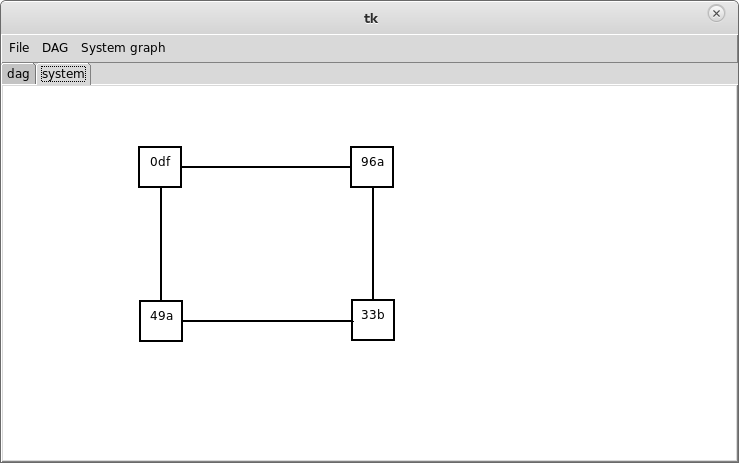
\includegraphics[width=\textwidth]{res/system_graph.png}
      \end{center}
      \caption{Інтерфейс користувача}
    \label{fig:gui}
    \end{figure}

\subsection{Внутрішнє представлення системи}
    Система представлена як група процесорів із заданою кількістю лінків. Система представлена класом System, він інкапсулює процесори, що представлені класом CPU, що також інкапсулює лінки (клас Link). Кожен процесор та лінк має можливість зберігати часові проміжки ScheduledTransmissionSegment та ScheduledTask, що репрезентують сегмент пересилання даних та сегмант обрахунку задачі відповідно.

Алгоритм перевірки на зв'язність: запускається алгоритм пошуку в глибину починаючи від першої вершини. Якщо пройдені вершини містять всі вершини графа, то граф зв'язний. Інтрфейс користувача для вводу графу системи показаний на рис. \ref{fig:system_graph}.
    \begin{figure}[h!]
      \begin{center}
        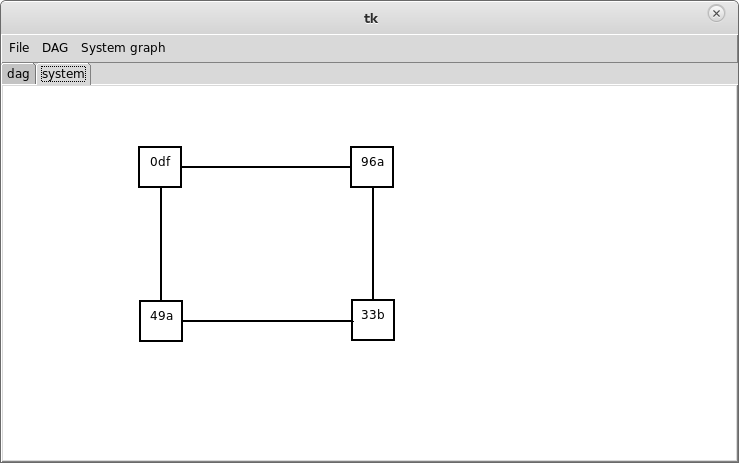
\includegraphics[width=\textwidth]{res/system_graph.png}
      \end{center}
      \caption{Інтерфейс користувача вводу задачі}
    \label{fig:system_graph}
    \end{figure}



    Для представлення графу задачі використовується кореневий клас DAG, що зберігає вершини у класах Node та зв'язки між ними у класах Edge.

    Алгоритм перевірки на ациклічності: запускається алгоритм пошуку в глибину починаючи від кожної вершини, генеруючи дерево вершин з коренем в поточній. Якщо в це дерево потрапляє вершина, яка вже в ньому присутня, то знайдений цикл. Інтрфейс користувача для вводу графу задачі показаний на рис. \ref{fig:gui_graph}.
    \begin{figure}[h!]
      \begin{center}
        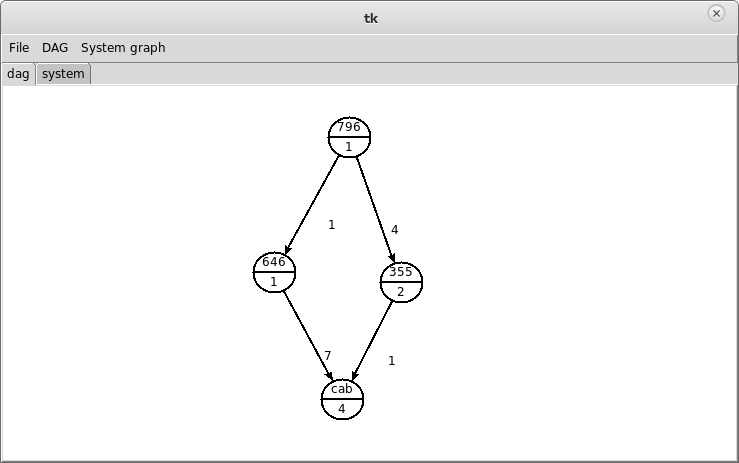
\includegraphics[width=\textwidth]{res/gui_graph.png}
      \end{center}
      \caption{Інтерфейс користувача вводу задачі}
    \label{fig:gui_graph}
    \end{figure}


\subsection{Алгоритми формування черги}
Алгоритми формування черги інкапсулюються в нащадків класу BaseQueueGenerationPolicy, в яких має бути реалізований метод get\_queue.

Алгоритм 3 формує чергу у порядку спадання критичного по часу шляхів до кінця графа задачі. Програма формує всі критичні шляхи у графі задачі і сортує їх за часом. Якщо час однаковий, то за номером вершини. Реалізація алгоритму у алгоритмі \ref{lst:a3}.

\begin{lstlisting}[language=Python,caption={Алгоритм 3},label=lst:a3]
class QueueGenerationPolicy3(BaseQueueGenerationPolicy):
    def get_queue(self, dag):
        paths = find_all_critical_paths(dag, forward=True, weight_based=True)

        def get_weight(item):
            node_id, (weight, path) = item
            return weight, node_id
        return [path[0] for path in sorted(paths.items(), key=get_weight, reverse=True)]

\end{lstlisting}

Алгоритм 4 формує чергу у порядку спадання критичного по кількості вершин шляхів до кінця графа задачі, а при рівних значеннях – в порядку спадання зв’язності вершин. Необхідно визначити всі критичні шляхи за кількістю вершин та відсортувати за кількістю, а при рівних - в спаданні зв'язності.  Реалізація алгоритму у алгоритмі \ref{lst:a4}.

\begin{lstlisting}[language=Python,caption={Алгоритм 4},label=lst:a4]
class QueueGenerationPolicy4(BaseQueueGenerationPolicy):
    def get_queue(self, dag):
        paths = find_all_critical_paths(dag, forward=True, weight_based=False)

        def get_weight(item):
            node_id, (weight, path) = item
            node = dag.nodes[node_id]
            return weight, len(dag.get_neighbours(node, forward=True) + dag.get_neighbours(node, forward=False))
        return [path[0] for path in sorted(paths.items(), key=get_weight, reverse=True)]

\end{lstlisting}

Алгоритм 16 формує чергу у порядку зростання критичного по часу шляхів вершин від початку графа задачі. Необхідно визначити критичні шляхи від початку графу та відсортувати за часом. Реалізація алгоритму у алгоритмі \ref{lst:a16}.

\begin{lstlisting}[language=Python,caption={Алгоритм 16},label=lst:a16]
class QueueGenerationPolicy16(BaseQueueGenerationPolicy):
    def get_queue(self, dag):
        paths = find_all_critical_paths(dag, forward=False, weight_based=True)

        def get_weight(item):
            node_id, (weight, path) = item
            return weight
        return [path[0] for path in sorted(paths.items(), key=get_weight)]

\end{lstlisting}

\subsection{Генерация випадкового графу задачі}    

Необхідно сформувати випадковий граф задачі за заданими параметрами. Програма надає можливість задання таких параметрів: (див. рис. \ref{fig:random_params})

    \begin{figure}[h!]
      \begin{center}
        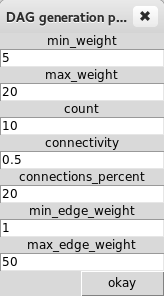
\includegraphics{res/random.png}
      \end{center}
      \caption{Інтерфейс задання параметрів випадкової задачі}
    \label{fig:random_params}
    \end{figure}

Алгоритм генерації випадкового графу:

\begin{enumerate}
    \item Генеруємо N вершин з випадковими вагами в заданих межах.
    \item Рахуємо суму вагів, за формулою кореляции рахуємо середню вагу дуги яку ми повинні отримати.
    \item По заданому відсотку кількості дуг та середному значенню, рахуємо їх кількість і генеруємо їх.
    \item Ваги дуг задаємо випадковим чином по нормальному розподілу, де mu = (очікувана сума) / (кількість дуг), а sigma = mu / 4, при цьому не дозволяємо вазі виходити за задані межі. При цьому, якщо середнє значення виходить за межі, то межі не враховуються.
    \item Якщо потрібна кореляція досягнута, але не всі ребра додані, зупиняємо додавання ребер.
    \item В останню дугу вагою записуємо необхідну різницю, щоб отримати потрібний коефіцієнт кореляції - без урахування меж.
\end{enumerate}

\begin{lstlisting}[language=Python,caption={Вихідний код генерації випадкового графу задачі},label=lst:random_dag]
    def generate(cls,
                 min_weight, max_weight,
                 count, connectivity, connections_percent,
                 min_edge_weight=None, max_edge_weight=None):
        graph = DAG()
        sum_weight = 0
        for i in range(count):
            weight = randint(min_weight, max_weight)
            graph.add_node(randint(0, 300), randint(0, 300), weight, str(i))
            sum_weight += weight

        sum_edges_weight = (sum_weight - connectivity*sum_weight) / connectivity

        max_edges_count = (count*(count-1)) / 2
        edges_count = int(connections_percent/100*max_edges_count)

        pairs = [(str(i), str(j)) for i in range(count) for j in range(i+1, count)]
        # 1 1 30 0.1 10 1 500
        sum_edges_weight_actual = 0
        last_edge = None
        added_edges_count = 0
        for source, target in sample(pairs, edges_count):
            average_edge_weight = max(1, ((sum_edges_weight - sum_edges_weight_actual) / (edges_count - added_edges_count)))
            weight = int(normalvariate(average_edge_weight, average_edge_weight/4))
            weight = norm_weight(weight, min_edge_weight, max_edge_weight, average_edge_weight)
            if sum_edges_weight - (sum_edges_weight_actual + weight) < 0:
                weight = max(1, int(sum_edges_weight - sum_edges_weight_actual))
                last_edge = graph.add_edge(source, target, weight)
                sum_edges_weight_actual += weight
                warnings.warn("Stopped, maximum reached: last edge weight was {} < {} < {}".
                              format(min_edge_weight, weight, max_edge_weight))
                break
            last_edge = graph.add_edge(source, target, weight)
            sum_edges_weight_actual += weight
            added_edges_count += 1
        else:
            weight = int(sum_edges_weight - sum_edges_weight_actual)
            if weight <= 0:
                weight = 1
            last_edge.weight = weight
            expected_weight = norm_weight(weight, min_edge_weight, max_edge_weight, average_edge_weight)
            if expected_weight != weight:
                warnings.warn("Last edge weight was out of bounds {} < {} < {}".
                              format(min_edge_weight, weight, max_edge_weight))

        graph.arrange()
        print("Correlation")
        print("actual: ", graph.correlatio(), "; expected: ", connectivity)
        return graph


\end{lstlisting}


\subsection{Процес моделювання}

Для моделювання написані тестові скрипти мовою Python, які запускають генерацію графу та планування в текстовому режимі без запуску графічної оболонки. Приклад скрипта наданий у лістингу \ref{lst:test}.

\begin{lstlisting}[language=Python,caption={Вихідний код скрипта порівняння 3 та 4 черги для алгоритму 6 з 3 лінками},label=lst:test]

def test(scale, connectivity, queue, scheduler_class, duplex, io_cpu, count=50):
    system_graph = get_thor_system()
    count = len(system_graph.nodes) * scale

    system = System(system_graph,
                    duplex=duplex,
                    has_io_cpu=io_cpu)
    router = DFSRouter(system_graph)

    k_accels = []
    k_efs = []
    for i in range(count):
        task_dag = DAG.generate(min_weight=5, max_weight=20,
                                count=count, connectivity=connectivity,
                                connections_percent=30)
        scheduler = scheduler_class(
            task_dag, system_graph, queue(), CohesionCPUPrioritizationPolicy(),
            system, router)
        scheduler.schedule_dag()
        k_accel = task_dag.duration_on_one_cpu() / system.duration()
        k_accels.append(k_accel)
        k_ef = k_accel / len(system._cpus)
        k_efs.append(k_ef)
    k_accel_avg = sum(k_accels) / len(k_accels)
    k_ef_avg = sum(k_efs) / len(k_efs)
    return k_accel_avg, k_ef_avg


def get_thor_system():
    system_graph = Graph()
    with open("saved/thor") as thor_file:
        system_graph_file = json.load(thor_file)
        Graph.deserialize(system_graph, system_graph_file, override_node={"weight": 3})
    return system_graph


def get_grid_system():
    system_graph = Graph()
    with open("saved/grid") as thor_file:
        system_graph_file = json.load(thor_file)
        Graph.deserialize(system_graph, system_graph_file)
    return system_graph


def loop(scale, queue, scheduler_class, duplex, io_cpu, count=50):
    print(queue.__name__ + " ", end='')
    print(scheduler_class.__name__ + " ", end='')
    if duplex:
        print("duplex; ", end='')
    else:
        print("no duplex; ", end='')
    if io_cpu:
        print("io_cpu; ", end='')
    else:
        print("no io_cpu; ", end='')
    print("scale %d:1" % scale)

    connectivity = 0.1
    data = []
    while connectivity < 1:
        print(">>", connectivity)
        accel, ef = test(scale=scale, connectivity=connectivity,
                         queue=queue,
                         scheduler_class=scheduler_class,
                         duplex=duplex, io_cpu=io_cpu,
                         count=count)
        data.append("%s, %s" % (accel, ef))

        connectivity += 0.1
    print("\n".join(data))


def main():
    warnings.simplefilter("ignore")
    scheduler_class = ModellingNeighbourScheduler
    duplex = True
    scale = 3
    loop(scale, queue=QueueGenerationPolicy3, scheduler_class=scheduler_class,
         duplex=duplex, io_cpu=True)
    print("================")
    loop(scale, queue=QueueGenerationPolicy4, scheduler_class=scheduler_class,
         duplex=duplex, io_cpu=True)
    print("================")

if __name__ == "__main__":
    main()

\end{lstlisting}


\subsection{Інструкція користувача}

Користувачу достіпні два екрани для вводу графів задачі (рис. \ref{fig:gui_graph_2}) та системи (рис. \ref{fig:system_graph_2}).

    \begin{figure}[h!]
      \begin{center}
        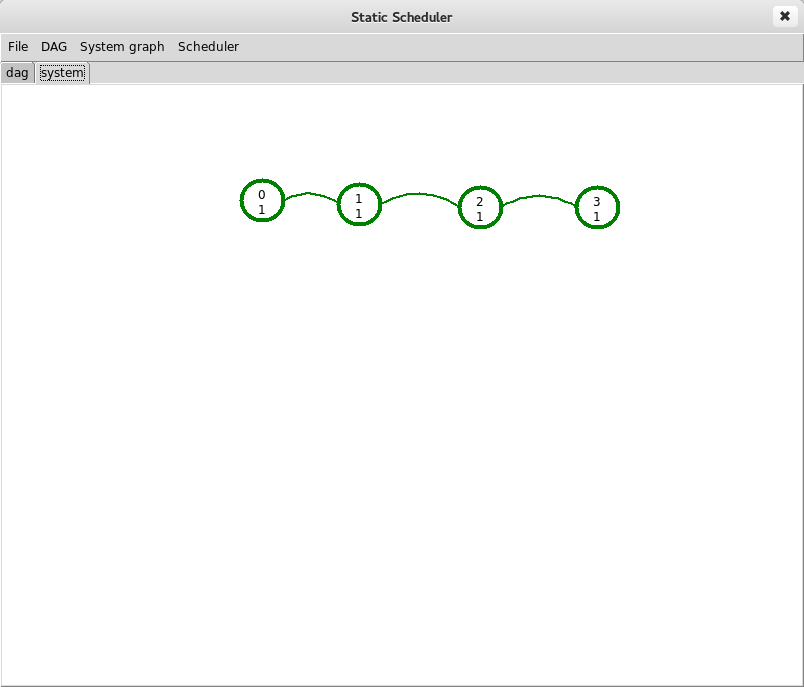
\includegraphics[width=\textwidth]{res/system_graph_new.png}
      \end{center}
      \caption{Інтерфейс користувача вводу системи}
    \label{fig:system_graph_2}
    \end{figure}

    \begin{figure}[h!]
      \begin{center}
        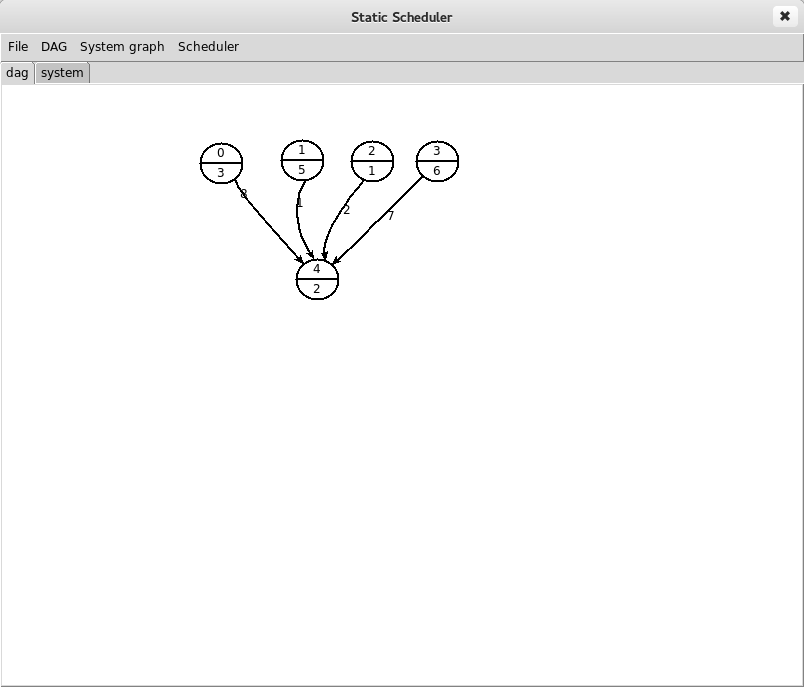
\includegraphics[width=\textwidth]{res/gui_graph_new.png}
      \end{center}
      \caption{Інтерфейс користувача вводу задачі}
    \label{fig:gui_graph_2}
    \end{figure}

Можливе зберігання та відкриття збережених графів задач та систем через меню File. Меню DAG надає можливість згенерувати випадковий граф а також виконувати операції із вже відкритим графом, такі як генерація трьох черг та пошук критичного шляху.

Для запуску процесу планування використовується пункт меню Scheduler -> Schedule.
Налаштування планувальника на рис. \ref{fig:sched_params}

    \begin{figure}[h!]
      \begin{center}
        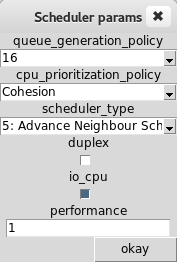
\includegraphics{res/sched_params.png}
      \end{center}
      \caption{Налаштування планувальника}
    \label{fig:sched_params}
    \end{figure}

Після запуску планувальника користувач побачить згенеровану діаграму Ганта на рис. \ref{fig:gantt}.

    \begin{figure}[h!]
      \begin{center}
        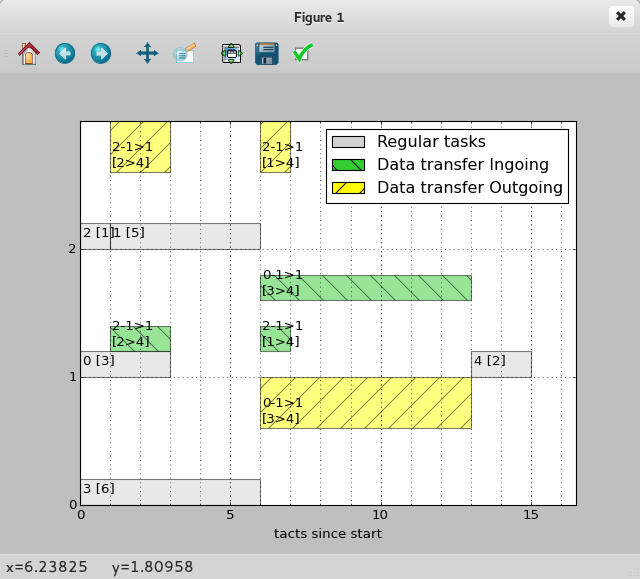
\includegraphics[width=\textwidth]{res/gantt.png}
      \end{center}
      \caption{Діаграма Ганта}
    \label{fig:gantt}
    \end{figure}

\section{Результати моделювання}
    \subsection{Порівняння алгоритмів планування}

    В програмі реалізовано 2 алгоритми планування та 3 алгоритми формування черг. Проаналізуємо роботу всіх варіантів комбінацій цих алгоритмів. Таких варіантів є 6. Для кожного варіанту прорахуємо декілька випадкових графів для кожної зв'язності від 0.1 до 0.9 із кроком 0.1.

    Візьмемо систему типу <<тор>> 3 порядку (рис. \ref{fig:thor}).

    \begin{figure}[h!]
      \begin{center}
        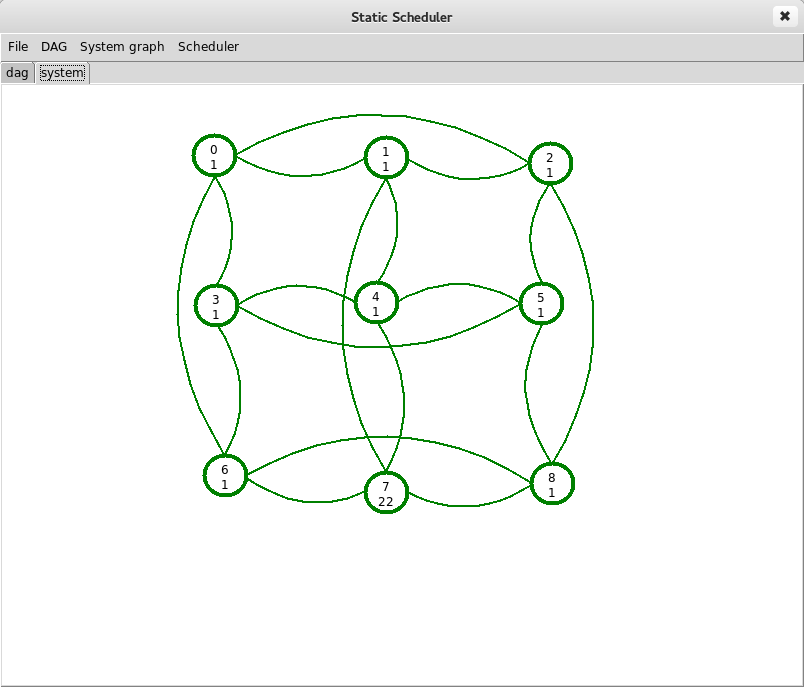
\includegraphics[width=\textwidth]{res/thor.png}
      \end{center}
      \caption{Топологія типу тор 3 порядку}
    \label{fig:thor}
    \end{figure}

    На кожному кроці зв'язності прорахуємо 15 випадкових графів та результуючий час усереднимо.
    Порахуємо коефіцієнт прискорення та коефіцієнт ефективності.

    Дуплексність присутня, процесор вводу виводу відсутній. Маштаб задачі до системи $1:1$

\begin{figure}[h]
  \begin{center}
    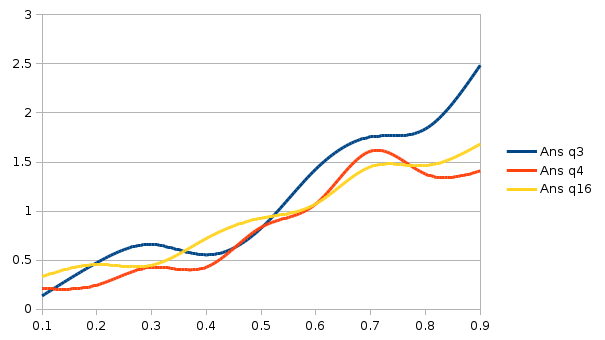
\includegraphics[width=\textwidth]{res/noio_ans.png}
  \end{center}
  \caption{Коефіцієнт прискорення алгоритму 5 без процесора вводу-виводу}
\label{fig:noio_ans}
\end{figure}

\begin{figure}[h]
  \begin{center}
    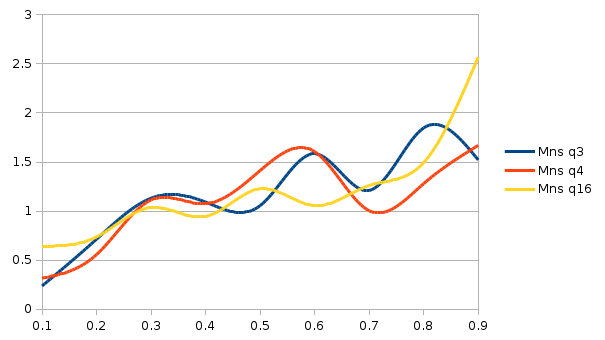
\includegraphics[width=\textwidth]{res/noio_mns.png}
  \end{center}
  \caption{Коефіцієнт прискорення алгоритму 6 без процесора вводу-виводу}
\label{fig:noio_mns}
\end{figure}

\begin{figure}[h]
  \begin{center}
    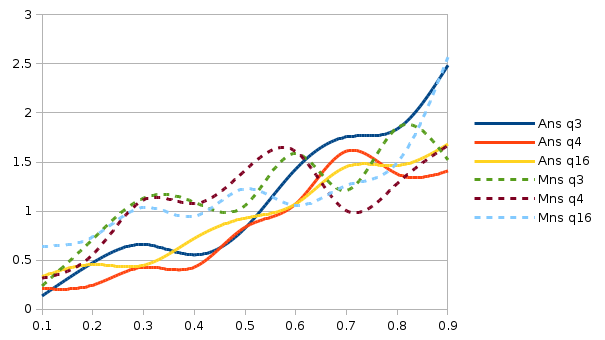
\includegraphics[width=\textwidth]{res/noio_both.png}
  \end{center}
  \caption{Суміщений графік коефіцієнтів прискорення алгоритмів 5 та 6 без процесора вводу-виводу}
\label{fig:noio_both}
\end{figure}

\begin{figure}[h]
  \begin{center}
    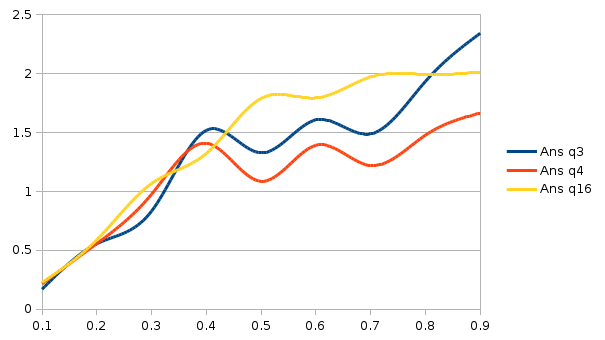
\includegraphics[width=\textwidth]{res/io_ans.png}
  \end{center}
  \caption{Коефіцієнт прискорення алгоритму 5 із процесором вводу-виводу}
\label{fig:io_ans}
\end{figure}

\begin{figure}[h]
  \begin{center}
    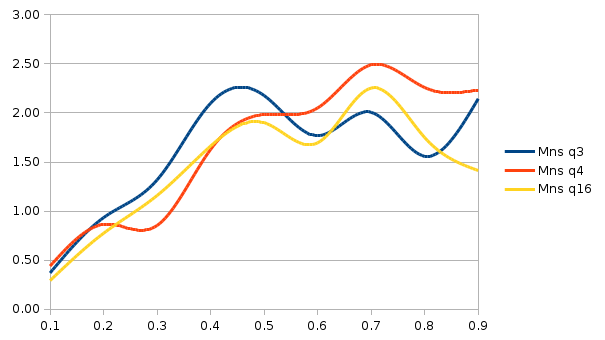
\includegraphics[width=\textwidth]{res/io_mns.png}
  \end{center}
  \caption{Коефіцієнт прискорення алгоритму 6 із процесором вводу-виводу}
\label{fig:io_mns}
\end{figure}

\begin{figure}[h]
  \begin{center}
    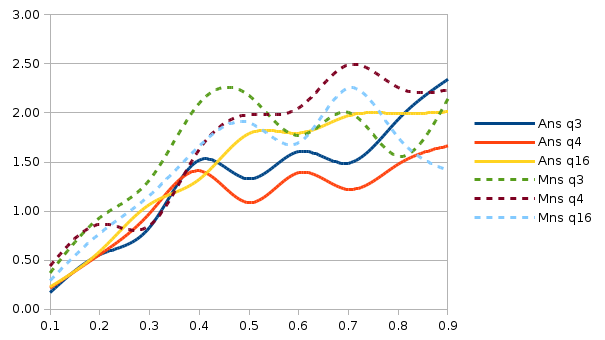
\includegraphics[width=\textwidth]{res/io_both.png}
  \end{center}
  \caption{Суміщений графік коефіцієнтів прискорення алгоритмів 5 та 6 із процесором вводу-виводу}
\label{fig:io_both}
\end{figure}


\begin{table}[H]
\caption{Алгоритм планування 5. Коефіцієнт прискорення. Процесор вводу виводу відсутній.}
\label{tab:big_table}
\centering
\begin{tabular}{lrrrrrrrrr}
\toprule
черга &   0.1 &   0.2 &   0.3 &   0.4 &   0.5 &   0.6 &   0.7 &   0.8 &   0.9 \\
\midrule
3 & 0.14 & 0.47 & 0.66 & 0.55 & 0.83 & 1.43 & 1.76 & 1.84 & 2.49 \\
4 & 0.21 & 0.25 & 0.43 & 0.43 & 0.84 & 1.07 & 1.61 & 1.38 & 1.41 \\
16 & 0.33 & 0.46 & 0.45 & 0.72 & 0.93 & 1.07 & 1.45 & 1.46 & 1.68 \\
\bottomrule
\end{tabular}
\end{table}

\begin{table}[H]
\caption{Алгоритм планування 6. Коефіцієнт прискорення. Процесор вводу виводу відсутній.}
\label{tab:big_table}
\centering
\begin{tabular}{lrrrrrrrrr}
\toprule
черга &   0.1 &   0.2 &   0.3 &   0.4 &   0.5 &   0.6 &   0.7 &   0.8 &   0.9 \\
\midrule
3 & 0.24 & 0.71 & 1.13 & 1.09 & 1.06 & 1.58 & 1.21 & 1.85 & 1.52 \\
4 & 0.32 & 0.56 & 1.11 & 1.08 & 1.41 & 1.61 & 1.00 & 1.28 & 1.67 \\
16 & 0.64 & 0.74 & 1.04 & 0.95 & 1.23 & 1.06 & 1.26 & 1.49 & 2.57 \\
\bottomrule
\end{tabular}
\end{table}


\begin{table}[H]
\caption{Алгоритм планування 5. Коефіцієнт ефективності. Процесор вводу виводу відсутній.}
\label{tab:big_table}
\centering
\begin{tabular}{lrrrrrrrrr}
\toprule
черга &   0.1 &   0.2 &   0.3 &   0.4 &   0.5 &   0.6 &   0.7 &   0.8 &   0.9 \\
\midrule
3 & 0.04 & 0.05 & 0.08 & 0.07 & 0.09 & 0.14 & 0.12 & 0.22 & 0.17 \\
4 & 0.02 & 0.03 & 0.05 & 0.05 & 0.09 & 0.12 & 0.18 & 0.15 & 0.16 \\
16 & 0.04 & 0.05 & 0.05 & 0.08 & 0.10 & 0.12 & 0.16 & 0.16 & 0.19 \\
\bottomrule
\end{tabular}
\end{table}

\begin{table}[H]
\caption{Алгоритм планування 6. Коефіцієнт ефективності. Процесор вводу виводу відсутній.}
\label{tab:big_table}
\centering
\begin{tabular}{lrrrrrrrrr}
\toprule
черга &   0.1 &   0.2 &   0.3 &   0.4 &   0.5 &   0.6 &   0.7 &   0.8 &   0.9 \\
\midrule
3 & 0.03 & 0.08 & 0.13 & 0.13 & 0.12 & 0.18 & 0.13 & 0.25 & 0.17 \\
4 & 0.04 & 0.06 & 0.12 & 0.12 & 0.16 & 0.18 & 0.11 & 0.14 & 0.19 \\
16 & 0.07 & 0.08 & 0.12 & 0.11 & 0.14 & 0.12 & 0.14 & 0.17 & 0.29 \\
\bottomrule
\end{tabular}
\end{table}

    Дуплексність присутня, процесор вводу виводу присутній. Маштаб задачі до системи $1:1$


\begin{table}[H]
\caption{Алгоритм планування 5. Коефіцієнт прискорення. Процесор вводу виводу присутній.}
\label{tab:big_table}
\centering
\begin{tabular}{lrrrrrrrrr}
\toprule
черга &   0.1 &   0.2 &   0.3 &   0.4 &   0.5 &   0.6 &   0.7 &   0.8 &   0.9 \\
\midrule
3 & 0.17 & 0.56 & 0.83 & 1.52 & 1.33 & 1.61 & 1.49 & 1.93 & 2.34 \\
4 & 0.22 & 0.56 & 0.98 & 1.41 & 1.09 & 1.39 & 1.22 & 1.48 & 1.67 \\
16 & 0.23 & 0.59 & 1.07 & 1.32 & 1.79 & 1.79 & 1.97 & 1.99 & 2.01 \\
\bottomrule
\end{tabular}
\end{table}

\begin{table}[H]
\caption{Алгоритм планування 6. Коефіцієнт прискорення. Процесор вводу виводу присутній.}
\label{tab:big_table}
\centering
\begin{tabular}{lrrrrrrrrr}
\toprule
черга &   0.1 &   0.2 &   0.3 &   0.4 &   0.5 &   0.6 &   0.7 &   0.8 &   0.9 \\
\midrule
3 & 0.37 & 0.73 & 1.02 & 2.10 & 2.18 & 1.77 & 2.01 & 1.56 & 2.14 \\
4 & 0.44 & 0.86 & 0.85 & 1.93 & 1.38 & 2.55 & 2.49 & 2.26 & 1.93 \\
16 & 0.29 & 0.77 & 1.16 & 1.66 & 1.90 & 1.70 & 2.25 & 1.75 & 1.41 \\
\bottomrule
\end{tabular}
\end{table}

\begin{table}[H]
\caption{Алгоритм планування 5. Коефіцієнт ефективності. Процесор вводу виводу присутній.}
\label{tab:big_table}
\centering
\begin{tabular}{lrrrrrrrrr}
\toprule
черга &   0.1 &   0.2 &   0.3 &   0.4 &   0.5 &   0.6 &   0.7 &   0.8 &   0.9 \\
\midrule
3 & 0.02 & 0.06 & 0.09 & 0.17 & 0.15 & 0.18 & 0.17 & 0.21 & 0.26 \\
4 & 0.02 & 0.06 & 0.11 & 0.16 & 0.12 & 0.15 & 0.14 & 0.16 & 0.19 \\
16 & 0.03 & 0.07 & 0.12 & 0.15 & 0.20 & 0.20 & 0.22 & 0.22 & 0.22 \\
\bottomrule
\end{tabular}
\end{table}

\begin{table}[H]
\caption{Алгоритм планування 6. Коефіцієнт ефективності. Процесор вводу виводу присутній.}
\label{tab:big_table}
\centering
\begin{tabular}{lrrrrrrrrr}
\toprule
черга &   0.1 &   0.2 &   0.3 &   0.4 &   0.5 &   0.6 &   0.7 &   0.8 &   0.9 \\
\midrule
3 & 0.04 & 0.08 & 0.11 & 0.23 & 0.24 & 0.20 & 0.22 & 0.17 & 0.24 \\
4 & 0.05 & 0.10 & 0.09 & 0.21 & 0.15 & 0.28 & 0.28 & 0.25 & 0.21 \\
16 & 0.03 & 0.09 & 0.13 & 0.18 & 0.21 & 0.19 & 0.25 & 0.19 & 0.16 \\
\bottomrule
\end{tabular}
\end{table}

Як можна сказати з графіку \ref{fig:noio_both} при відсутності процесору вводу/виводу приблизно до зв'язності 0.6 найбільш ефективними є алгоритми з моделюванням. На ділянці 0.1-0.6 правильним вибором буде алгоритм 6 із 4 алгоритмом черги.

Після 0.6 немає чіткої різниці між алгоритмами. Тому, зважаючи на вимірювання часу із наступного розділу, при зв'язності більшій ніж 0.6 рекомендовано використовувати алгоритм 5 сусіднього призначення із чергою 3, як найбільш ефективного по часу та дещо більшого за коефіцієнтом прискорення за інші алгоритми.

З графіку \ref{fig:io_both} при наявності процесору вводу/виводу аналіз дає дещо інші результати. На всій ділянці від 0.1 до 0.9 найбільш ефективними є алгоритми 6 з моделюванням. При цьому на проміжку 0.1-0.5 це алгоритм 6 з чергою 3, а на проміжку 0.6-0.9 це алгоритм 6 з чергою 4.

Судячи з графіків, варіант із процесорами вводу-виводу є більш ефективним. Для подальшого аналізу оберемо систему із процесорами вводу/виводу, і проаналізуємо роботу алгоритмів 6-3 та 6-4 на проміжках 0.1-0.5 та 0.6-0.9 відповідно на іншій топології та з іншими параметрами системи.

\subsection{Порівняння часу роботи алгоритмів планування}

Для порівняння часу роботи 5 та 6 алгоритмів зробимо замір часу для кожної зв'язності від 0.1 до 0.9 при увімкненому дуплексі та процесорах вводу/виводу.
Необхідності перевіряти час роботи на всіх алгоритмах формування черги немає, тому що вони еквівалентні за складністю та не внесуть змін у статистику.

\begin{table}[H]
\caption{Час роботи алгоритмів (msec)}
\label{tab:big_table}
\centering
\begin{tabular}{llrrrrrrrrr}
\toprule
Алгоритм & Черга &   0.1 &   0.2 &   0.3 &   0.4 &   0.5 &   0.6 &   0.7 &   0.8 &   0.9 \\
\midrule
5 & 3 & 391 & 320 & 299 & 280 & 264 & 258 & 251 & 251 & 252 \\
6 & 3 & 513 & 387 & 340 & 326 & 312 & 302 & 299 & 298 & 295 \\
\bottomrule
\end{tabular}
\end{table}

\subsection{Вивчення впливу топології}

Для порівняння результатів візьмемо схожу на тор топологію - решітка 3 порядку (рис. \ref{fig:grid}).

    \begin{figure}[h!]
      \begin{center}
        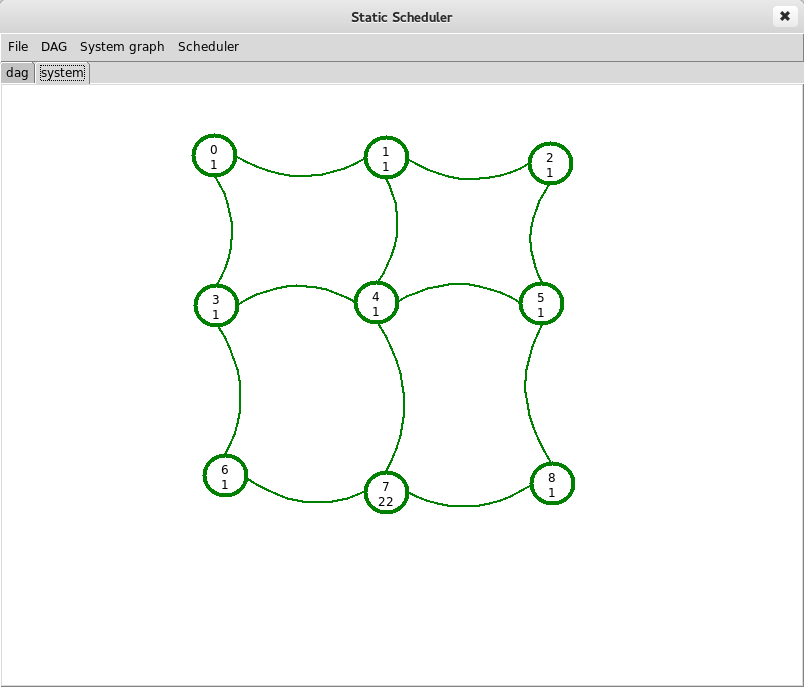
\includegraphics[width=\textwidth]{res/grid.png}
      \end{center}
      \caption{Топологія типу решітка 3 порядку}
    \label{fig:grid}
    \end{figure}

\section{Выводы}
    При виконанні курсового проекту розроблений програмний продукт для моделювання MPP систем у різних конфігураціях.

    Досліджені алгоритми сусіднього призначення із моделюванням та без моделювання. Ці алгоритми досліджені з використанням 3х алгоритмів формування черг.

    Показано, що алгоритм з моделюванням (6) дає найкращі результати, при використанні черги 3 від 0.1 до 0.5 показника зв'язності та при використанні черги 4 від 0.6 до 0.9.

    Суміщений алгоритм 6-3 та 6-4 на двох проміжках досліджений на різних системах: з топологією тор та решітка, з 1, 2 та 3 лінками на процесорах та із різними маштабами заданих задач, $1:1$, $1:2$, $1:3$.

    Показано, що на маштабі $1:3$ із 2 лінками на процесорах у топології тор алгоритм дає найбільш високий результат.
\section{Список использованной литературы}
\begin{enumerate}
    \item Конспект лекций по предмету "Программное обеспечение компьютерных систем"
    \item Русанова О. В. Программное обеспечение компьютерных систем //Особенности программирования и компиляции. Учебное пособие. Киев,«Корнійчук. – 2003.
    \item Олифер В. и др. Компьютерные сети. – 2010.
    \item Grayson J. E. Python Tkinter Programming. – 2011.
    \item Hunter J. D. Matplotlib: A 2D graphics environment //Computing in science and engineering. – 2007. – Т. 9. – №. 3. – С. 90-95.
\end{enumerate}

\ESKDappendix{}{Вихідний код}
\singlespacing
%\addtolength{\hoffset}{2cm}
\lstinputlisting{res/src.py}

\end{document}
